% Appendix B

\chapter{JSON parser in C} % Main appendix title

\label{AppendixB} % For referencing this appendix elsewhere, use \ref{AppendixA}

\lhead{Appendix B. \emph{JSON Parser in C}} % This is for the header on each page - perhaps a shortened title
%--------------------------------------------------------------------
\lstdefinestyle{DOS}
{
    backgroundcolor=\color{black},
    basicstyle=\scriptsize\color{white}\ttfamily
    numbers=none,
    numbersep=8pt,                   % how far the line-numbers are from the code
    numberstyle=\tiny\color{white}, % the style that is used for the line-numbers
    stepnumber=1                    % the step between two line-numbers. If it's 1, each line will be numbered
}
%----------------------------------------------------------------------------------------
\lstdefinestyle{C}
{
  morekeywords={export}
}
%----------------------------------------------------------------------------------------
This appendix will explains how to implemente the JSON parser in C language using library JSON-c.
%----------------------------------------------------------------------------------------
\section{Objective of JSON Parser}
The objective of our JSON parser is to parser a JSON file generated by Luup HTTP Request. The website \href{http://www.wikibooks.org}{Online JSON Viewer} can be used to visualise the JSON file. Below is a JSON example of our JSON file named \textbf{status.json}:

\begin{figure}[htbp]
	\centering
		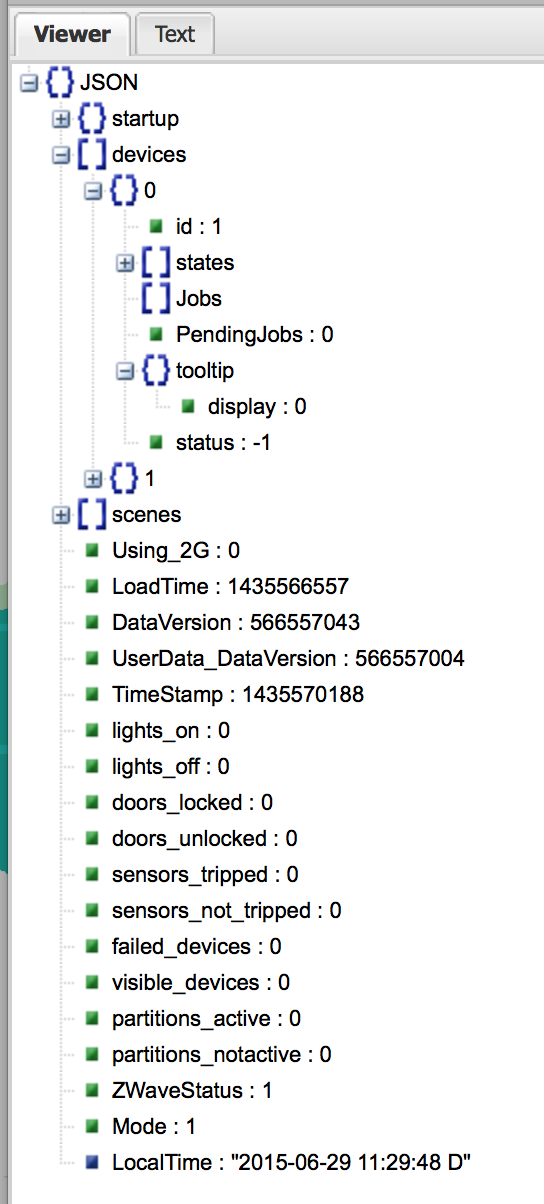
\includegraphics[width=8cm]{Figures/jsonviewer.png}
	\caption[JSON File in JSON Viewer Online]{JSON File in JSON Viewer Online}
\end{figure}

In order to import the data into TR-069, the JSON format should be convert to Z-Wave format which is like:
\begin{lstlisting}[mathescape]
    ZWave.devices.1.id 1
    ZWave.devices.1.states.1.id 208
    ZWave.devices.1.states.1.service urn:micasaverde-com:serviceId:ZWaveNetwork1
    ZWave.devices.1.states.1.value 1
    ZWave.devices.1.states.2.id 209
    ZWave.devices.1.states.2.service urn:micasaverde-com:serviceId:ZWaveNetwork1
    ZWave.devices.1.states.2.variable UseMR
    ZWave.devices.1.states.2.value 1
    ZWave.devices.1.states.3.id 210
    ZWave.devices.1.states.3.service urn:micasaverde-com:serviceId:ZWaveNetwork1
    ZWave.devices.1.states.3.variable LimitNeighbors
    ZWave.devices.1.states.3.value 0
    ZWave.devices.1.states.4.id 211
    ZWave.devices.1.states.4.service urn:micasaverde-com:serviceId:ZWaveNetwork1
    ZWave.devices.1.states.4.variable LastDongleBackup
\end{lstlisting}

First part is the name and second is the value.
%----------------------------------------------------------------------------------------------
\section{JSON Format Charcteristic}
JSON is built on two structures:

\begin{itemize}
  \item A collection of name/value pairs. In various languages, this is realized as an object, record, struct, dictionary, hash table, keyed list, or associative array.
  \item An ordered list of values. In most languages, this is realized as an array, vector, list, or sequence.
\end{itemize}
An object is an unordered set of name/value pairs. An object begins with \{ (left brace) and ends with \} (right brace). Each name is followed by : (colon) and the name/value pairs are separated by , (comma).

\begin{figure}[htbp]
	\centering
		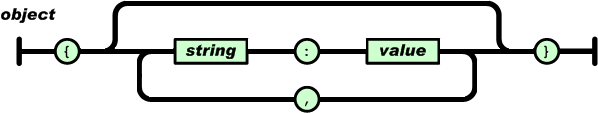
\includegraphics[width=12cm]{Figures/jsonobject.png}
	\caption[JSON Object Strcture]{JSON Object Strcture}
\end{figure}

An array is an ordered collection of values. An array begins with [ (left bracket) and ends with ] (right bracket). Values are separated by , (comma).
\begin{figure}[htbp]
	\centering
		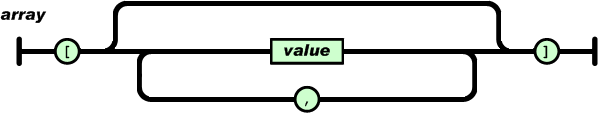
\includegraphics[width=12cm]{Figures/jsonarray.png}
	\caption[JSON Array Strcture]{JSON Array Strcture}
\end{figure}

In the array case, the index must be added after the last level( e.g ZWave.devices.1.states.2.id 209). The parser works in a iterative way.

\section{Implementation of JSON Parser}

At first, we set a buffer to store the path for each parameter. Then use the json-c libary function \textit{json_object_from_file} to save all the file content into a JSON object:

\begin{lstlisting}[mathescape]
    char path_json[70] = "ZWave.";    //set the buffer to save the name of parameter, also as the head

    struct json_object* jobj = json_object_from_file(fichierLu);  //fichierLu set to the file path to parse

    _jsonParser(path_json, jobj);  //jobj is the json object will be parsed
\end{lstlisting}


\textit{_jsonParser} is the private function to parse the JSON object. There is a essential json-c libary function called \textit{json_object_object_foreach(jobj, key, val)}, it allows to traverse each object in the json object. Before that, the current path should be added into a string.

\begin{lstlisting}[mathescape]
    /*Parsing the json object*/
    void _jsonParser(char *path, json_object * jobj)
    {
       enum json_type type;

       char parse_path[100];                          //define the local variable for path
       strcpy(parse_path,path);

       json_object_object_foreach(jobj, key, val)   /*Passing through every array element*/
       {
          type = json_object_get_type(val);
          switch (type)
          {
             case json_type_boolean:
             case json_type_double:
             case json_type_int:
             case json_type_string:  _printJsonValue(parse_path, val, key);
                                     break;

             case json_type_object:  sprintf(&parse_path[strlen(parse_path)], "%s.",key );
                                     jobj = json_object_object_get(jobj, key);
                                     _jsonParser(parse_path, jobj);
                                     break;

             case json_type_array:   _jsonParseArray(jobj, key, parse_path);
                                     break;
          }
       }
    }
\end{lstlisting}

If the object parsed is a value, jump to the \textit{_printJsonValue} function to save the value in buffer table. If it's a object, redo this function. If it's a array, goto the \textit{_jsonParseArray} function.

\begin{lstlisting}[mathescape]
    /*Parsing the json array*/
    void _jsonParseArray( json_object *jobj, char *key, char *path)
    {
       void _jsonParser(char *path, json_object * jobj); /*Forward Declaration*/
       enum json_type type;

       char array_path[100];                            //define the local variable for path
       strcpy(array_path,path);
       json_object * jvalue;


       json_object *jarray = jobj; /*Simply get the array*/

       if(key) {jarray = json_object_object_get(jobj, key); /*Getting the array if it is a key value pair*/}

       int arraylen = json_object_array_length(jarray); /*Getting the length of the array*/
       int i;

       sprintf(&array_path[strlen(array_path)],"%s.",key);

       sprintf(&array_path[strlen(array_path)],"x.");   //fill the path with x. for instance

       for (i=0; i< arraylen; i++)
       {
          jvalue = json_object_array_get_idx(jarray, i); /*Getting the array element at position i*/
          type = json_object_get_type(jvalue);

          if( i <= 9 )
             sprintf(&array_path[strlen(array_path)-2], "%d.",i + 1 );  //replace the 2 last char x.
          else
             sprintf(&array_path[strlen(array_path)-3], "%d.",i + 1 );  //replace the 3 last char xx.


          if (type == json_type_array)
             _jsonParseArray(jvalue, NULL,array_path);
          else if (type == json_type_object)
             _jsonParser(array_path, jvalue);
          else
             _printJsonValue(array_path, jvalue, NULL);
       }
    }
\end{lstlisting}

The main difficulty of parse a array is to add the index. The solution is to add .x at every beginning of Array parse, and then replace the .x according to different object type.

\begin{lstlisting}[mathescape]
    /*At the end of each iteration, write the name/value pair to a 2D table*/
    void _printJsonValue( char* path, json_object *jobj, char *key)
    {
      enum json_type type;

      type = json_object_get_type(jobj); /*Getting the type of the json object*/

      char* value_buffer;
      value_buffer = (char*)malloc(150 * sizeof(char));

      char* paramKey;
      paramKey = (char*)malloc((strlen(path)+strlen(key)) * sizeof(char));

      strcpy(paramKey,path);         //build the JSON object name string
      strcat(paramKey,key);

      switch (type)
      {
          case json_type_boolean: sprintf(value_buffer,"%s",json_object_get_boolean(jobj)? "true": "false");
                                  sdataParameterList[indiceValueStruct] = DM_ENG_newSystemParameterValueStruct(paramKey, value_buffer, NULL);
                                  break;
          case json_type_double:  sprintf(value_buffer,"%lf",json_object_get_double(jobj));
                                  sdataParameterList[indiceValueStruct] = DM_ENG_newSystemParameterValueStruct(paramKey, value_buffer, NULL);
                                  break;
          case json_type_int:     sprintf(value_buffer,"%d",json_object_get_int(jobj));
                                  sdataParameterList[indiceValueStruct] = DM_ENG_newSystemParameterValueStruct(paramKey, value_buffer, NULL);
                                  break;
          case json_type_string:  value_buffer = strdup(json_object_get_string(jobj));
                                  sdataParameterList[indiceValueStruct] = DM_ENG_newSystemParameterValueStruct(paramKey, value_buffer, NULL);
                                  break;
      }
      free(value_buffer);
      indiceValueStruct++;
    }
\end{lstlisting}

On the \textit{_printJsonValue} function, each element in the buffe table is a TR-069 \textit{System Parameter Value Struct} using the TR-069 Client API default function \textit{DM_ENG_newSystemParameterValueStruct}.
